
%(BEGIN_QUESTION)
% Copyright 2011, Tony R. Kuphaldt, released under the Creative Commons Attribution License (v 1.0)
% This means you may do almost anything with this work of mine, so long as you give me proper credit

In this process, steam is introduced into ``stripping'' vessel C-7 to help remove volatile sulfur compounds from ``sour'' water.  The temperature of the stripped gases exiting the tower's top is controlled by a pneumatic temperature control loop.  Unfortunately, this loop seems to have a problem.

Temperature indicating recorder TIR-21 registers 304 degrees Fahrenheit, while temperature indicating controller TIC-21 registers 285 degrees Fahrenheit.  The calibrated range of TT-21 is 100 to 350 degrees Fahrenheit.  A technician connects a test gauge to the pneumatic signal line and reads a pressure of 12.8 PSI:

$$\includegraphics[width=15.5cm]{i0007rx01.eps}$$

Which instrument is faulty: the transmitter, the recorder, or the controller, or is it impossible to tell from what little information is given here?

\underbar{file i03541}
%(END_QUESTION)





%(BEGIN_ANSWER)

We know the indicating controller (TIC-21) must be miscalibrated, because the pneumatic signal pressure of 12.8 PSI agrees with the recorder's indication of 304 degrees F.

%(END_ANSWER)





%(BEGIN_NOTES)

\filbreak \vskip 20pt \vbox{\hrule \hbox{\strut \vrule{} {\bf Virtual Troubleshooting} \vrule} \hrule}

\noindent
{\bf Predicting the effect of a given fault:} present each of the following faults to the students, one at a time, having them comment on all the effects each fault would produce.

\begin{itemize}
\item{} PC-115 left in manual mode
\item{} Isolation valve to PC-115 left in shut position
\item{} PV-115 has a positive calibration error (open further than it should be)
\item{} TT-21 has positive calibration error (outputs too high of a signal)
\item{} Bypass valve around TV-21 left open
\item{} LY-12 has negative calibration error (outputs too low of a signal)
\item{} Bypass valve around LV-12 left open
\item{} FT-28 fails with a low signal
\item{} FT-27 fails with a high signal
\end{itemize}


\vskip 10pt


\noindent
{\bf Identifying possible/impossible faults:} present symptoms to the students and then have them determine whether or not a series of suggested faults could account for all the symptoms, explaining {\it why} or {\it why not} for each proposed fault:

\begin{itemize}
\item{} 
\item{} 
\item{} 
\end{itemize}


\vskip 10pt


\noindent
{\bf Determining the utility of given diagnostic tests:} imagine the ??? fails ??? in this system (but don't tell this to students!).  Present the operator's observation(s) to the students, have them consider possible faults and diagnostic strategies, and then propose the following diagnostic tests one by one.  Have students rate the value of each test, determining whether or not each test would give us useful information (i.e. tell us something we don't already know).  Also have students describe what re

\begin{itemize}
\item{} {\it }
\item{}  -- {\bf Yes/No}
\item{}  -- {\bf Yes/No}
\end{itemize}


\vskip 10pt


\noindent
{\bf Diagnosing a fault based on given symptoms:} imagine the ??? fails ??? in this system (but don't tell this to students!).  Present the operator's observation(s) to the students, have them consider possible faults and diagnostic strategies, and then tell them the results of tests they propose based on the following symptoms, until they have properly identified the nature and location of the fault:

\begin{itemize}
\item{} {\it }
\item{} 
\item{} 
\end{itemize}

%INDEX% Measurement, temperature: troubleshooting (realistic P&ID shown)
%INDEX% Process: sour water stripping tower (realistic P&ID shown)

%(END_NOTES)

